\chapter{Results}
\section{Segmentation performance}

\pgfplotstableread[col sep=comma]{../src/data/evaluation.csv}\loadedtable

\begin{table}[ht]
\centering
\caption{Segmentation performance on easy images.}
\pgfplotstabletypeset[
    col sep=comma,
    columns={model,accuracy,precision,recall,specificity,f1,iou},
    columns/model/.style={string type,column name=Model},
    columns/accuracy/.style={fixed,precision=3,column name=Accuracy},
    columns/precision/.style={fixed,precision=3,column name=Precision},
    columns/recall/.style={fixed,precision=3,column name=Recall},
    columns/specificity/.style={fixed,precision=3,column name=Specificity},
    columns/f1/.style={fixed,precision=3,column name=$F_1$},
    columns/iou/.style={fixed,precision=3,column name=IoU},
    row predicate/.code={
        \pgfplotstablegetelem{\pgfplotstablerow}{difficulty}\of{\loadedtable}
        \edef\temp{\pgfplotsretval}
        \def\match{easy}
        \ifx\temp\match
        \else
            \pgfplotstableuserowfalse
        \fi
    },
    every head row/.style={before row=\toprule,after row=\midrule},
    every last row/.style={after row=\bottomrule}
]{\loadedtable}
\end{table}

\begin{table}[ht]
\centering
\caption{Segmentation performance on medium images.}
\pgfplotstabletypeset[
    col sep=comma,
    columns={model,accuracy,precision,recall,specificity,f1,iou},
    columns/model/.style={string type,column name=Model},
    columns/accuracy/.style={fixed,precision=3,column name=Accuracy},
    columns/precision/.style={fixed,precision=3,column name=Precision},
    columns/recall/.style={fixed,precision=3,column name=Recall},
    columns/specificity/.style={fixed,precision=3,column name=Specificity},
    columns/f1/.style={fixed,precision=3,column name=$F_1$},
    columns/iou/.style={fixed,precision=3,column name=IoU},
    row predicate/.code={
        \pgfplotstablegetelem{\pgfplotstablerow}{difficulty}\of{\loadedtable}
        \edef\temp{\pgfplotsretval}
        \def\match{medium}
        \ifx\temp\match
        \else
            \pgfplotstableuserowfalse
        \fi
    },
    every head row/.style={before row=\toprule,after row=\midrule},
    every last row/.style={after row=\bottomrule}
]{\loadedtable}
\end{table}

\begin{table}[ht]
\centering
\caption{Segmentation performance on hard images.}
\pgfplotstabletypeset[
    col sep=comma,
    columns={model,accuracy,precision,recall,specificity,f1,iou},
    columns/model/.style={string type,column name=Model},
    columns/accuracy/.style={fixed,precision=3,column name=Accuracy},
    columns/precision/.style={fixed,precision=3,column name=Precision},
    columns/recall/.style={fixed,precision=3,column name=Recall},
    columns/specificity/.style={fixed,precision=3,column name=Specificity},
    columns/f1/.style={fixed,precision=3,column name=$F_1$},
    columns/iou/.style={fixed,precision=3,column name=IoU},
    row predicate/.code={
        \pgfplotstablegetelem{\pgfplotstablerow}{difficulty}\of{\loadedtable}
        \edef\temp{\pgfplotsretval}
        \def\match{hard}
        \ifx\temp\match
        \else
            \pgfplotstableuserowfalse
        \fi
    },
    every head row/.style={before row=\toprule,after row=\midrule},
    every last row/.style={after row=\bottomrule}
]{\loadedtable}
\end{table}

\begin{figure}[htbp]
\centering

\begin{subfigure}{0.3\textwidth}
    \centering
    \fbox{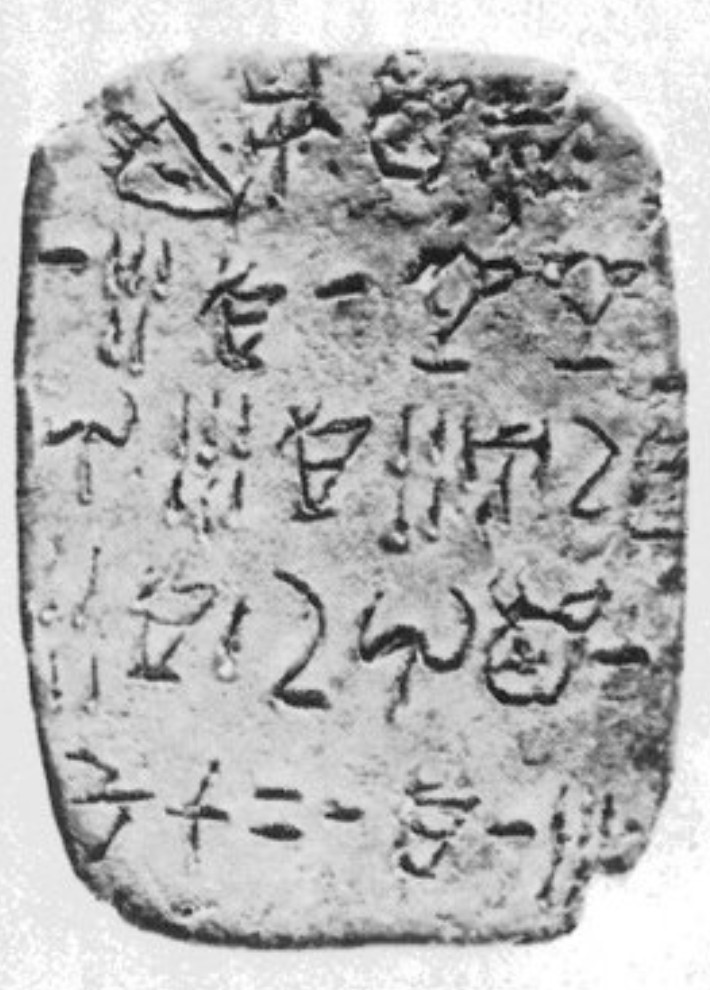
\includegraphics[width=\linewidth]{../src/data/raw/easy/HT118.jpg}}
    \caption{Raw}
\end{subfigure}
\hfill
\begin{subfigure}{0.3\textwidth}
    \centering
    \fbox{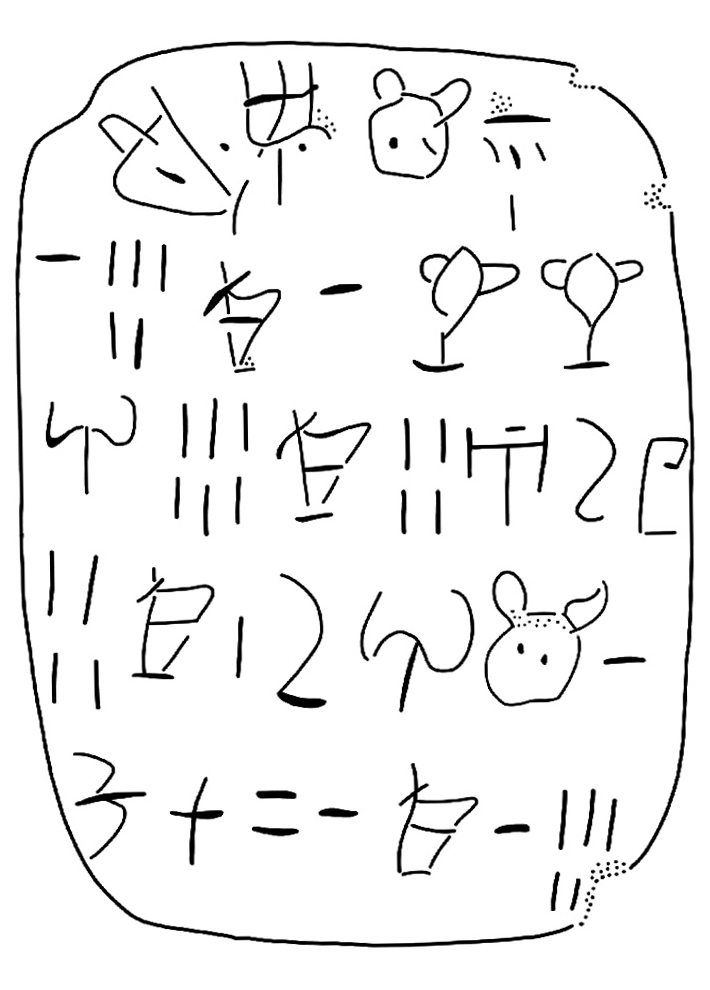
\includegraphics[width=\linewidth]{../src/data/ground_truth/registered/HT118.jpg}}
    \caption{Ground Truth}
\end{subfigure}
\hfill
\begin{subfigure}{0.3\textwidth}
    \centering
    \fbox{\includegraphics[width=\linewidth]{../src/data/scribed/HT118-Otsu.jpg}}
    \caption{Otsu}
\end{subfigure}

\vspace{0.5em}

\begin{subfigure}{0.3\textwidth}
    \centering
    \fbox{\includegraphics[width=\linewidth]{../src/data/scribed/HT118-Gaussian.jpg}}
    \caption{Gaussian}
\end{subfigure}
\hfill
\begin{subfigure}{0.3\textwidth}
    \centering
    \fbox{\includegraphics[width=\linewidth]{../src/data/scribed/HT118-CannyFill.jpg}}
    \caption{CannyFill}
\end{subfigure}
\hfill
\begin{subfigure}{0.3\textwidth}
    \centering
    \fbox{\includegraphics[width=\linewidth]{../src/data/scribed/HT118-GrabCutAutoBox.jpg}}
    \caption{GCautobox}
\end{subfigure}

\vspace{0.5em}

\begin{subfigure}{0.3\textwidth}
    \centering
    \fbox{\includegraphics[width=\linewidth]{../src/data/scribed/HT118-GrabCutAutoBrush.jpg}}
    \caption{GCautobrush}
\end{subfigure}
\hfill
\begin{subfigure}{0.3\textwidth}
    \centering
    \fbox{\includegraphics[width=\linewidth]{../src/data/scribed/HT118-Sam.jpg}}
    \caption{mSAM}
\end{subfigure}
\hfill
\begin{subfigure}{0.3\textwidth}
    \centering
    \fbox{\includegraphics[width=\linewidth]{../src/data/scribed/HT118-SamAutoBox.jpg}}
    \caption{mSAMautobox}
\end{subfigure}

\caption{Comparison of segmentation outputs from different models against the raw image and ground truth.}
\label{fig:model_comparison}

\end{figure}

\begin{figure}
\centering
\begin{tikzpicture}
\begin{axis}[
ybar,
bar width=12pt,
width=12cm,
height=7cm,
ylabel={IoU},
ymin=0,
ymax=0.45,
symbolic x coords={Otsu,Gaussian,CannyFill,GCautobox,GCautobrush,mSAM,mSAMautobox},
xtick=data,
xticklabel style={rotate=45,anchor=east},
]
\addplot table [x=model,y=iou,col sep=comma] {\loadedtable};
\end{axis}
\end{tikzpicture}
\caption{IoU performance per model. Each bar shows the overall performance, while the horizontal lines within each bar indicate the IoU values obtained for the easy, medium, and hard difficulty subsets.}
\end{figure}

\section{Automation evaluation}
\section{Workflow efficiency evaluation}